\documentclass[11pt,a4paper]{scrartcl}

\usepackage[T1]{fontenc}
\usepackage{lmodern}
\usepackage[margin=18mm]{geometry}
\usepackage{amsmath,amssymb}
\usepackage{booktabs,array}
\usepackage{microtype}
\usepackage{xcolor}
\usepackage{tikz}
\usetikzlibrary{arrows.meta,calc,fit,positioning,shapes.geometric}

\DeclareMathOperator{\JSR}{JSR}

\definecolor{BaseBlue}{HTML}{2F6C99}
\definecolor{HybridGreen}{HTML}{2D7A4B}
\definecolor{PerfOrange}{HTML}{A9581C}
\definecolor{SoftBlue}{HTML}{EAF3F8}
\definecolor{SoftGreen}{HTML}{EAF5EE}
\definecolor{SoftOrange}{HTML}{FFF2E7}
\definecolor{SoftGray}{HTML}{F5F5F5}
\definecolor{Ink}{HTML}{1F2933}

\setlength{\parindent}{0pt}
\setlength{\parskip}{0.45em}
\renewcommand{\arraystretch}{1.18}

\tikzset{
  every picture/.style={line width=0.72pt},
  treebox/.style={
    draw=Ink!75,
    rounded corners=1.5pt,
    align=center,
    font=\scriptsize,
    minimum width=17mm,
    minimum height=7mm,
    inner sep=2.2pt,
    fill=white
  },
  rootbox/.style={treebox, fill=SoftBlue},
  closedbox/.style={treebox, fill=SoftGreen, draw=HybridGreen!80},
  exactbox/.style={treebox, fill=SoftOrange, draw=PerfOrange!85},
  flowbox/.style={
    draw=Ink!75,
    rounded corners=2pt,
    align=center,
    font=\scriptsize,
    text width=25mm,
    minimum height=8mm,
    inner sep=3pt,
    fill=white
  },
  flowbase/.style={flowbox, fill=SoftBlue},
  flowstrict/.style={flowbox, fill=SoftGreen},
  flowperf/.style={flowbox, fill=SoftOrange},
  flowarrow/.style={-{Latex[length=2.1mm]}, draw=Ink!70},
  tinylabel/.style={font=\scriptsize, fill=white, inner sep=1pt},
  ax/.style={draw=Ink!50, -{Latex[length=2mm]}},
  pt/.style={circle, draw=Ink, fill=white, minimum size=3.3mm, inner sep=0pt},
  impt/.style={circle, draw=HybridGreen!80!black, fill=SoftGreen, minimum size=3.3mm, inner sep=0pt}
}

\newcommand{\matthree}[9]{%
  \begin{pmatrix}
    #1 & #2 & #3\\
    #4 & #5 & #6\\
    #7 & #8 & #9
  \end{pmatrix}}

\begin{document}

\begin{center}
  {\Large\bfseries Low-dimensional IPA hybrid certificate example}\\[0.25em]
  {\small Example \texttt{controlled\_d3\_n2\_seed2\_a0.35\_s0.45\_c0.25}. Values are from the generated profiling artifact.}
\end{center}

\section{Starting matrices and problem formulation}

The matrix family is
\[
\mathcal A=\{A_1,A_2\}\subset \mathbb R^{3\times 3}.
\]
For this example the invariant-polytope algorithm is initialized with the spectrum-maximizing product
\[
\Pi=A_1,\qquad \rho(\Pi)=1,\qquad \lambda=1.
\]
The computational problem is to certify
\[
\JSR(\mathcal A)=1.
\]
The matrices used by the run are
\[
A_1=
\matthree
{0.28608433}{0.03859008}{0.03387308}
{0.03859008}{0.99003830}{-0.07403809}
{0.03387308}{-0.07403809}{0.33637737},
\]
\[
A_2=
\matthree
{0.16701638}{-0.00114923}{0.02347436}
{0.05850404}{0.20641451}{0.02404550}
{0.01739058}{0.03269350}{0.18344411}.
\]
Since \(A_1\) has spectral radius one, the hybrid certificate uses \(A_1\) as the generator.
The stored infinite-path leaf word is
\[
(-1,2).
\]
Here the negative index \(-1\) denotes the generator direction associated with \(A_1\), and the positive index \(2\) denotes the original matrix \(A_2\).

\section{Used starting vertices}

The first vertex is the leading eigenvector of \(A_1\). Two extra vertices are added explicitly.
\[
v_1=
\begin{pmatrix}
-0.04853357\\
-0.99293274\\
 0.10830080
\end{pmatrix},
\qquad
v_2=e_2=
\begin{pmatrix}0\\1\\0\end{pmatrix},
\qquad
v_3=e_3=
\begin{pmatrix}0\\0\\1\end{pmatrix}.
\]

The following diagram shows the initial vertices and their one-step images under \(A_1\) and \(A_2\).
The picture uses the \((x_2,x_3)\)-projection, so it is a diagnostic plot rather than a geometric proof.

\begin{center}
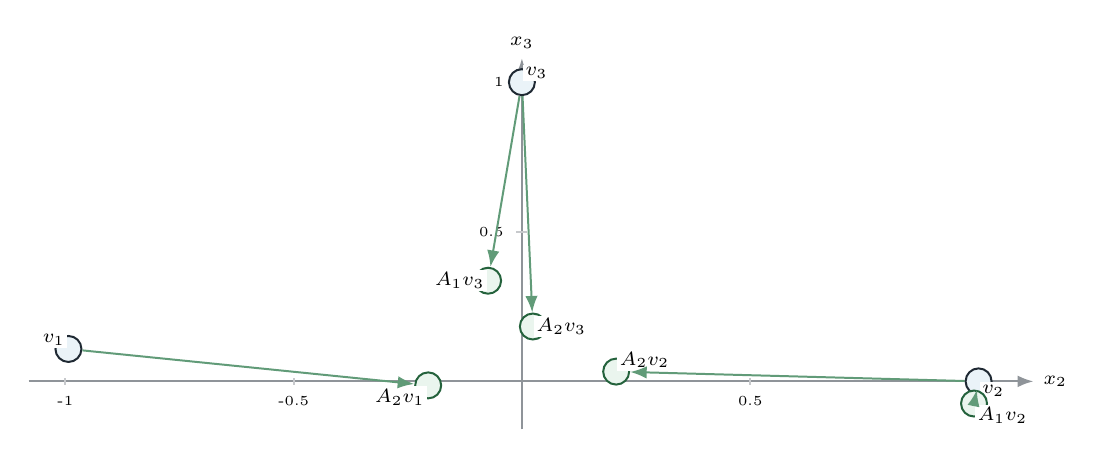
\begin{tikzpicture}[x=58mm,y=38mm]
  \draw[ax] (-1.08,0) -- (1.12,0) node[right,font=\scriptsize] {$x_2$};
  \draw[ax] (0,-0.16) -- (0,1.08) node[above,font=\scriptsize] {$x_3$};
  \foreach \y/\lab in {-1/-1, -0.5/-0.5, 0.5/0.5, 1/1} {
    \draw[Ink!25] (\y,-0.012) -- (\y,0.012);
    \node[font=\tiny,below] at (\y,-0.018) {\lab};
  }
  \foreach \z/\lab in {0.5/0.5, 1/1} {
    \draw[Ink!25] (-0.012,\z) -- (0.012,\z);
    \node[font=\tiny,left] at (-0.018,\z) {\lab};
  }

  \node[pt,fill=SoftBlue] (vone) at (-0.9929,0.1083) {};
  \node[tinylabel,anchor=south east] at (vone) {$v_1$};
  \node[pt,fill=SoftBlue] (vtwo) at (1,0) {};
  \node[tinylabel,anchor=north west] at (vtwo) {$v_2$};
  \node[pt,fill=SoftBlue] (vthree) at (0,1) {};
  \node[tinylabel,anchor=south west] at (vthree) {$v_3$};

  \node[impt] (a1v1) at (-0.2052,-0.0134) {};
  \node[tinylabel,anchor=north east] at (a1v1) {$A_2v_1$};
  \draw[flowarrow,HybridGreen!75] (vone) -- (a1v1);

  \node[impt] (a1v2) at (0.9900,-0.0740) {};
  \node[tinylabel,anchor=north west] at (a1v2) {$A_1v_2$};
  \draw[flowarrow,HybridGreen!75] (vtwo) -- (a1v2);

  \node[impt] (a2v2) at (0.2064,0.0327) {};
  \node[tinylabel,anchor=south west] at (a2v2) {$A_2v_2$};
  \draw[flowarrow,HybridGreen!75] (vtwo) -- (a2v2);

  \node[impt] (a1v3) at (-0.0740,0.3364) {};
  \node[tinylabel,anchor=east] at (a1v3) {$A_1v_3$};
  \draw[flowarrow,HybridGreen!75] (vthree) -- (a1v3);

  \node[impt] (a2v3) at (0.0240,0.1834) {};
  \node[tinylabel,anchor=west] at (a2v3) {$A_2v_3$};
  \draw[flowarrow,HybridGreen!75] (vthree) -- (a2v3);
\end{tikzpicture}
\end{center}

\section{How the certificate is evaluated for three IPA versions}

The baseline run uses ordinary IPA behavior. It generates vertices and evaluates exact polytope norms.
The two hybrid runs construct the same initial cyclic trees but then try to close frontier vertices by the infinite-path certificate.
The summary below is measured from the same profiling run.

\begin{center}
\begin{tabular}{lrrrrrr}
\toprule
Mode & vertices & generated & exact calls & exact points & hybrid closed & hybrid checks\\
\midrule
baseline & 7 & 13 & 2 & 4 & 0 & 0\\
strict & 3 & 5 & 0 & 0 & 5 & 5\\
performance & 3 & 5 & 0 & 0 & 2 & 2\\
\bottomrule
\end{tabular}
\end{center}

For a candidate frontier vertex \(x\), the hybrid code evaluates the finite part, the limiting branch, and a tail bound.
The recorded result has the form
\[
\text{closed if}\qquad
\texttt{max\_upper\_norm}(x)<1
\quad\text{and the stored tail bound is below the admissible threshold.}
\]
In this example every hybrid check closes.
Strict mode evaluates every frontier vertex.
Performance mode batches the checks and stops after the cheaper checks already close the necessary frontier vertices.

\begin{center}
\begin{tabular}{lrrrrr}
\toprule
Mode & tree & vertex & max upper norm & tail \(N\) & tail bound\\
\midrule
strict & 1 & 2 & 0.04640145 & 0 & 0.37997383\\
strict & 2 & 2 & 0.22752354 & 0 & 0.37017767\\
strict & 2 & 3 & 0.05685588 & 1 & 0.20662863\\
strict & 3 & 2 & 0.65556671 & 2 & 0.42480253\\
strict & 3 & 3 & 0.37907819 & 2 & 0.24092434\\
\midrule
performance & 2 & 2 & 0 & 0 & 0.37017767\\
performance & 3 & 2 & 0 & 2 & 0.42480253\\
\bottomrule
\end{tabular}
\end{center}

\section{Used trees}

The three cyclic trees are rooted at \(v_1,v_2,v_3\).
The edge labels are the indices of \(A_1\) and \(A_2\).
The baseline has to grow trees \(T_2\) and \(T_3\) beyond depth one.
The hybrid runs keep only the shallow frontier and certify it through the leaf word \((-1,2)\).

\subsection*{Baseline trees}

\begin{center}
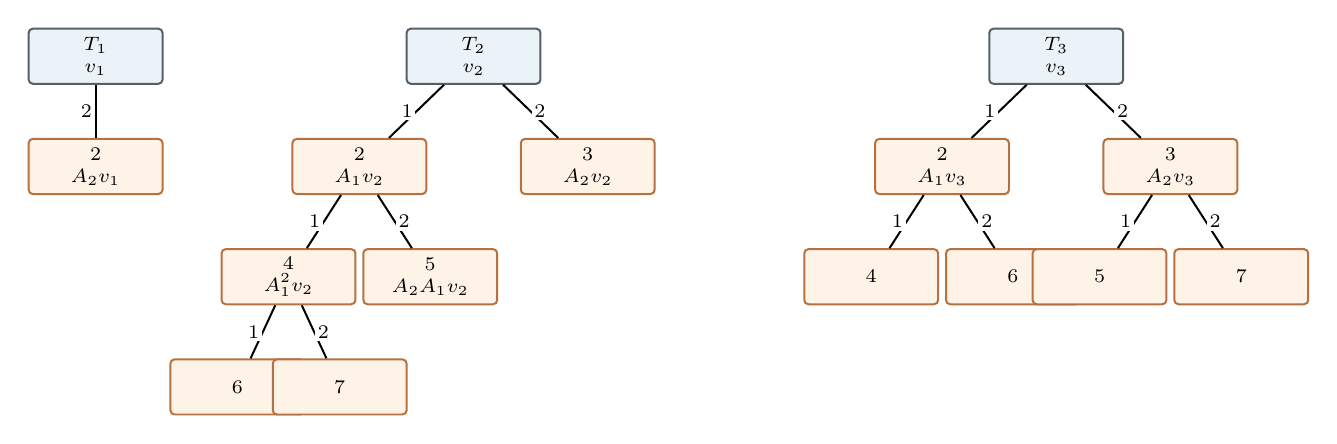
\begin{tikzpicture}[level distance=14mm,
  level 1/.style={sibling distance=29mm},
  level 2/.style={sibling distance=18mm},
  level 3/.style={sibling distance=13mm}]
  \node[rootbox] (b1r) {$T_1$\\$v_1$}
    child {node[exactbox] {$2$\\$A_2v_1$} edge from parent node[tinylabel,left] {$2$}};

  \begin{scope}[xshift=48mm]
  \node[rootbox] {$T_2$\\$v_2$}
    child {node[exactbox] {$2$\\$A_1v_2$}
      child {node[exactbox] {$4$\\$A_1^2v_2$}
        child {node[exactbox] {$6$} edge from parent node[tinylabel,left] {$1$}}
        child {node[exactbox] {$7$} edge from parent node[tinylabel,right] {$2$}}
        edge from parent node[tinylabel,left] {$1$}}
      child {node[exactbox] {$5$\\$A_2A_1v_2$} edge from parent node[tinylabel,right] {$2$}}
      edge from parent node[tinylabel,left] {$1$}}
    child {node[exactbox] {$3$\\$A_2v_2$} edge from parent node[tinylabel,right] {$2$}};
  \end{scope}

  \begin{scope}[xshift=122mm]
  \node[rootbox] {$T_3$\\$v_3$}
    child {node[exactbox] {$2$\\$A_1v_3$}
      child {node[exactbox] {$4$} edge from parent node[tinylabel,left] {$1$}}
      child {node[exactbox] {$6$} edge from parent node[tinylabel,right] {$2$}}
      edge from parent node[tinylabel,left] {$1$}}
    child {node[exactbox] {$3$\\$A_2v_3$}
      child {node[exactbox] {$5$} edge from parent node[tinylabel,left] {$1$}}
      child {node[exactbox] {$7$} edge from parent node[tinylabel,right] {$2$}}
      edge from parent node[tinylabel,right] {$2$}};
  \end{scope}
\end{tikzpicture}
\end{center}

\subsection*{Hybrid trees}

\begin{center}
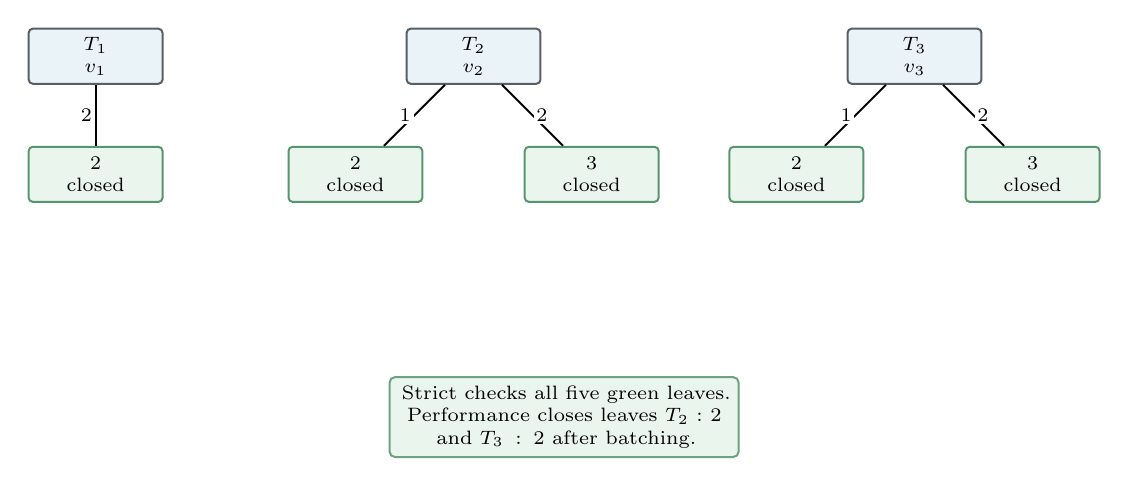
\begin{tikzpicture}[level distance=15mm,
  level 1/.style={sibling distance=30mm}]
  \node[rootbox] {$T_1$\\$v_1$}
    child {node[closedbox] {$2$\\closed} edge from parent node[tinylabel,left] {$2$}};

  \begin{scope}[xshift=48mm]
  \node[rootbox] {$T_2$\\$v_2$}
    child {node[closedbox] {$2$\\closed} edge from parent node[tinylabel,left] {$1$}}
    child {node[closedbox] {$3$\\closed} edge from parent node[tinylabel,right] {$2$}};
  \end{scope}

  \begin{scope}[xshift=104mm]
  \node[rootbox] {$T_3$\\$v_3$}
    child {node[closedbox] {$2$\\closed} edge from parent node[tinylabel,left] {$1$}}
    child {node[closedbox] {$3$\\closed} edge from parent node[tinylabel,right] {$2$}};
  \end{scope}

  \node[draw=HybridGreen!70, fill=SoftGreen, rounded corners=2pt, align=center,
        font=\scriptsize, text width=42mm, below=22mm of current bounding box.south] (legend)
        {Strict checks all five green leaves.\\Performance closes leaves \(T_2:2\) and \(T_3:2\) after batching.};
\end{tikzpicture}
\end{center}

\section{Call flow}

The next diagram uses the measured MATLAB profiler call graph.
Times are wall-clock times attributed to the corresponding call edge in the low-dimensional run.
The baseline spends time in exact norm work.
The hybrid runs enter \texttt{ipa\_hybrid\_filter\_vertices}; strict checks each tree separately, while performance uses a batched path.

\begin{center}
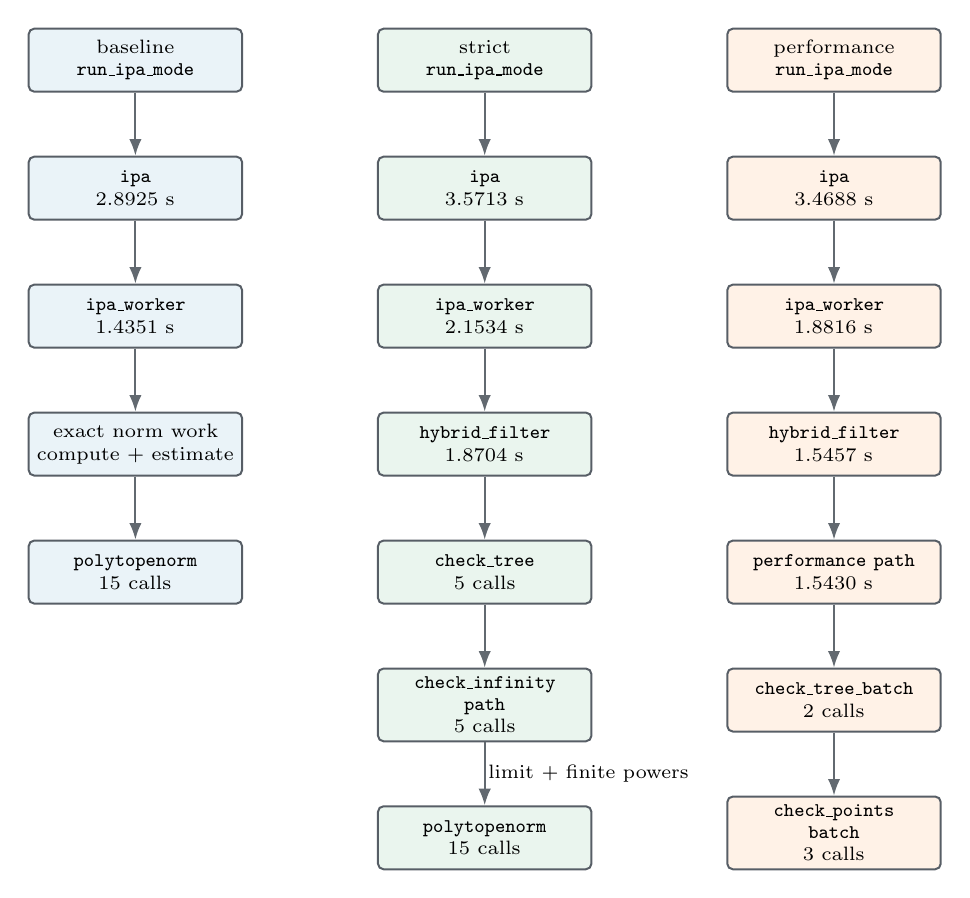
\begin{tikzpicture}[node distance=8mm and 8mm]
  \node[flowbase] (b0) {baseline\\\texttt{run\_ipa\_mode}};
  \node[flowbase, below=of b0] (b1) {\texttt{ipa}\\2.8925 s};
  \node[flowbase, below=of b1] (b2) {\texttt{ipa\_worker}\\1.4351 s};
  \node[flowbase, below=of b2] (b3) {exact norm work\\compute + estimate};
  \node[flowbase, below=of b3] (b5) {\texttt{polytopenorm}\\15 calls};

  \draw[flowarrow] (b0) -- (b1);
  \draw[flowarrow] (b1) -- (b2);
  \draw[flowarrow] (b2) -- (b3);
  \draw[flowarrow] (b3) -- (b5);

  \node[flowstrict, right=17mm of b0] (s0) {strict\\\texttt{run\_ipa\_mode}};
  \node[flowstrict, below=of s0] (s1) {\texttt{ipa}\\3.5713 s};
  \node[flowstrict, below=of s1] (s2) {\texttt{ipa\_worker}\\2.1534 s};
  \node[flowstrict, below=of s2] (s3) {\texttt{hybrid\_filter}\\1.8704 s};
  \node[flowstrict, below=of s3] (s4) {\texttt{check\_tree}\\5 calls};
  \node[flowstrict, below=of s4] (s5) {\texttt{check\_infinity}\\\texttt{path}\\5 calls};
  \node[flowstrict, below=of s5] (s6) {\texttt{polytopenorm}\\15 calls};

  \draw[flowarrow] (s0) -- (s1);
  \draw[flowarrow] (s1) -- (s2);
  \draw[flowarrow] (s2) -- (s3);
  \draw[flowarrow] (s3) -- (s4);
  \draw[flowarrow] (s4) -- (s5);
  \draw[flowarrow] (s5) -- node[tinylabel,right] {limit + finite powers} (s6);

  \node[flowperf, right=17mm of s0] (p0) {performance\\\texttt{run\_ipa\_mode}};
  \node[flowperf, below=of p0] (p1) {\texttt{ipa}\\3.4688 s};
  \node[flowperf, below=of p1] (p2) {\texttt{ipa\_worker}\\1.8816 s};
  \node[flowperf, below=of p2] (p3) {\texttt{hybrid\_filter}\\1.5457 s};
  \node[flowperf, below=of p3] (p4) {\texttt{performance path}\\1.5430 s};
  \node[flowperf, below=of p4] (p5) {\texttt{check\_tree\_batch}\\2 calls};
  \node[flowperf, below=of p5] (p6) {\texttt{check\_points}\\\texttt{batch}\\3 calls};

  \draw[flowarrow] (p0) -- (p1);
  \draw[flowarrow] (p1) -- (p2);
  \draw[flowarrow] (p2) -- (p3);
  \draw[flowarrow] (p3) -- (p4);
  \draw[flowarrow] (p4) -- (p5);
  \draw[flowarrow] (p5) -- (p6);
\end{tikzpicture}
\end{center}

\begin{center}
\begin{tabular}{lrrrr}
\toprule
Mode & wall time & profiler functions & line hits & exact norm points\\
\midrule
baseline & 2.89299 s & 473 & 120244 & 4\\
strict & 3.57157 s & 517 & 171573 & 0\\
performance & 3.46920 s & 525 & 119110 & 0\\
\bottomrule
\end{tabular}
\end{center}

\end{document}
